\documentclass[14pt]{beamer}
\usepackage[utf8]{inputenc}
\usetheme{Singapore}
\usepackage{amsmath}
\usepackage{amsfonts}
\usepackage{amssymb}
\usepackage{graphicx}
\usepackage[demo]{graphicx}
\usepackage{caption}
\usepackage{subcaption}
%\author[María Gabriela Ertola Navajas]{Gabriela Ertola Navajas}
\title{ECONOM\'{I}A I (E010)}
%\setbeamercovered{transparent} 
%\setbeamertemplate{navigation symbols}{} 
%\institute{} 
\date{3 de agosto, 2020} 
%\subject{} 
\setbeamertemplate{navigation symbols}{}

\begin{document}

\begin{frame}
\titlepage
\centering

\includegraphics[scale=0.25]{Magistrales O_2020/Figures/logoUDESA.jpg} 
\end{frame}

\begin{frame}
\frametitle{Profesores, mails y horarios de consulta}
\begin{itemize}
    \item Gaby (gertolanavajas@udesa.edu.ar)
    \item Fede (fsturzenegger@udesa.edu.ar)
    \begin{itemize}
    Viernes de 14 a 15 hs.
    \end{itemize} \vspace{2mm}
    \item Natalia (npecorari@udesa.edu.ar)
    \begin{itemize}
    Miércoles de 12 a 13 hs. 
    \end{itemize} \vspace{2mm}
    \item Victoria (vluca@udesa.edu.ar)
    \begin{itemize}
    Lunes de 11 a 12 hs.
    \end{itemize}
    \item Tomás (talvarezkuhnle@udesa.edu.ar)
    \begin{itemize}
    Jueves de 15 a 16 hs. 
    \end{itemize}
\end{itemize}
Deberán contactarse por mail enviando la/s pregunta/s especificas que tengan para coordinar la reunión.
\end{frame}

\begin{frame}
\frametitle{Objetivos}
\begin{itemize}
    \item Introducir a los estudiantes al estudio de la economía y a la manera de pensar y ver el mundo de los economistas.
    \begin{itemize}
        \item Familiarizar a los estudiantes con las herramientas y métodos de la disciplina.
        \item Ayudarlos a pensar como economistas. 
    \end{itemize}
\item Desarrollar la capacidad de los estudiantes para:
    \begin{itemize}
        \item Pensar en forma crítica los problemas sociales que afectan a las economías modernas.
        \item Evaluar qué herramientas analíticas son las más adecuadas para lidiar con esos problemas.
        \item Integrar teoría y análisis empírico 
    \end{itemize}    
\end{itemize}
\end{frame}

\begin{frame}
\frametitle{Modalidad de trabajo}
\begin{itemize}
    \item ¡Este curso implica mucho trabajo! Pero...  \vspace{2mm}
    \item ¡Vamos a trabajar en temas muy interesantes e útiles!  \vspace{2mm}
    \item ¿Cómo es una clase magistral? 
        \begin{itemize}
            \item Presentación de temas, con discusión sobre ellos
            \item Considerable interacción profesor-alumnos
            \item Llámennos por el nombre, trataremos de hacer lo mismo
        \end{itemize}
\end{itemize}
\end{frame}

\begin{frame}
\frametitle{Clases}
26 clases magistrales a lo largo del semestre 
\begin{itemize}
        \item 13 antes del receso de parciales, 13 en la segunda parte
        \item ¿Cuándo?
            \begin{itemize}
            \item Lunes de 12:40 a 14:20 hs
            \item Jueves de 14:30 a 16:10 hs
            \end{itemize}
\end{itemize}
13 tutoriales, una vez por semana, empezando la semana que viene 
\begin{itemize}
 \item ¿Cuándo?
        \begin{itemize}
            \item Lunes de 14:30 a 16:10 hs. (Tomás)
            \item Viernes de 14:30 a 16:10 hs. (Natalia)
            \item Viernes de 16:20 a 18:00 hs. (Natalia)
            \item Viernes de 16:20 a 18:00 hs. (Victoria)
        \end{itemize}
\end{itemize}
\end{frame}

\begin{frame}
\frametitle{Cronograma primera mitad}
\centering
\includegraphics[scale=0.4]{Magistrales O_2020/calendarioparte1campus.jpg}
\end{frame}

\begin{frame}
\frametitle{Cronograma segunda mitad}
\centering
\includegraphics[scale=0.4]{Magistrales O_2020/calendarioparte2campus.jpg}
\end{frame}

\begin{frame}
\frametitle{Materiales: TODO en el Campus Virtual}
Materiales principales
\begin{itemize}
    \item Slides de las magistrales (antes de la clase)
    \item Ejercitaciones para las tutoriales
    \item Lecturas
    \begin{itemize}
        \item Vamos a seguir un fascinante libro de texto, muy reciente, y open-access online: \\
        CORE Team [2017]:  \textit{The Economy: Economics for a Changing World}
        \item Ver calendario de lecturas para cada sesión
        \end{itemize}
\end{itemize}
\end{frame}

\begin{frame}
\frametitle{\href{http://www.core-econ.org}{Proyecto CORE} \url{http://www.core-econ.org}}
\centering
\includegraphics[scale=0.45]{Magistrales O_2020/core.jpg}
\end{frame}

\begin{frame}
\frametitle{Calendario de lecturas}
\centering
\includegraphics[scale=0.6]{Magistrales O_2020/biblio.jpg}
\end{frame}

\begin{frame}
\frametitle{Calendario de lecturas}
\centering
\includegraphics[scale=0.6]{Magistrales O_2020/biblio2.jpg}
\end{frame}

\begin{frame}
\frametitle{Evaluación del curso ($N_{curso}$)}
\begin{itemize}
    \item Promedio de pop-quizzes ($N_{quizzes}$, 10\% de $N_{curso}$) \vspace{2mm}
    \item Trabajo en tutoriales ($N_{tutorial}$, 20\% de $N_{curso}$) \vspace{2mm}
    \item Exámenes escritos (70\% de $N_{curso}$)
    \begin{itemize} \vspace{2mm}
        \item Dos parciales ($N_{parcial 1}$, $N_{parcial 2}$ 35\% de $N_{curso}$) \vspace{2mm}
        \item Un final ($N_{final}$, 70\% de $N_{curso}$)
    \end{itemize}    
\end{itemize}
\end{frame}

\begin{frame}
\frametitle{Pop-quizzes}
12 exámenes sorpresa (muy cortos) \vspace{2mm}
\begin{itemize}
    \item Sólo 4 minutos, al principio de la lección, en horario en punto!
    \item 6 preguntas, sobre la lectura del día
    \item Multiple choice y/o verdadero/falso
    \item Calculando la nota:
\end{itemize}
    \vspace{2mm}
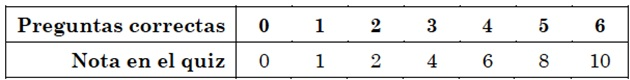
\includegraphics[scale=0.6]{Magistrales O_2020/notaquizzes.jpg}
\begin{itemize}
    \item ¿Cómo me preparo?
    \item El primero no será sorpresa... ¡es el lunes que viene!
\end{itemize}
\end{frame}

\begin{frame}
\frametitle{Tutoriales}
Se va a trabajar alrededor de ejercitaciones \begin{itemize}
    \item Disponibles en el Campus Virtual
    \begin{itemize}
            \item Típicamente, con dos semanas de antelación
        \end{itemize}
    \item Ejercicios
        \begin{itemize}
            \item Algunos para hacer y entregar antes de la tutorial
            \item Los demás se van a hacer y discutir en clase
        \end{itemize}
    \item Materiales
        \begin{itemize}
            \item En general, sólo el libro de texto
            \item Trabajo en la computadora
        \end{itemize}
\end{itemize} 
    \vspace{2mm}
Evaluación tutorial 
\begin{itemize} 
        \item Resolución de la guía de ejercicios (50\%)
        \item Trabajo grupal (40\%)
        \item Nota concepto (10\%)
    \end{itemize}   
\end{frame}

\begin{frame}
\frametitle{Exámenes}
\begin{itemize}
    \item Los exámenes (muy probablemente) serán virtuales
        \begin{itemize}
            \item Se incluirán preguntas multiple choice, verdaderos/falsos con discusión, y ejercicios
            \item Los parciales evaluarán los temas discutidos en cada mitad del curso y tendrán más preguntas que las que se tienen que responder
            \item El final cubre toda la materia y no habrá posibilidad de elección
        \end{itemize}
    \item Accediendo al segundo parcial
        \begin{itemize}
            \item Todos deben participar del primer parcial
            \item El acceso al segundo es sólo para los que hayan obtenido una ‘nota umbral’ igual o mayor a seis ($N_{umbral} \geq 6$)
        \end{itemize}
\end{itemize}
\end{frame}

\begin{frame}
\frametitle{Estructura exámenes}
\centering
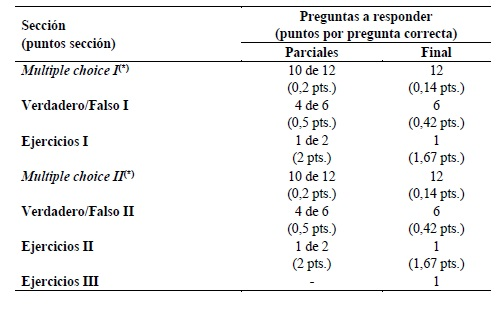
\includegraphics[scale=0.8]{Magistrales O_2020/examenes.jpg}
\end{frame}

\begin{frame}
\frametitle{Nota "umbral"}
\begin{itemize}
    \item Este curso contiene un alto número de puntos de evaluación a lo largo del semestre:
        \begin{itemize}
            \item 12 pop-quizzes
            \item 13 tutoriales (con distintas evaluaciones dentro)
            \item Exámenes escritos
        \end{itemize}
    \item La nota ‘umbral’ es simplemente un indicador del trabajo durante el semestre que puede dar acceso a ‘privilegios’ de evaluación
        \begin{itemize}
            \item Es el promedio (no ponderado) de la evaluación en quizzes, primer parcial y tutoriales:  
        \end{itemize}
        $N_{umbral}=1/3N_{quizzes}+1/3N_{tutorial}+1/3N_{parcial 1}$
\end{itemize}
\end{frame}

\begin{frame}
\frametitle{Nota del curso}
\begin{itemize}
    \item Para los que hayan accedido al segundo parcial 
\end{itemize}
\small{$N_{curso}=0,1N_{quizzes}+0,2N_{tutorial}+0,35N_{parcial 1}+0,35N_{parcial 2}$}
\vspace{2mm}
\begin{itemize}
    \item Para los que hayan accedido al final
\end{itemize}
\small{$N_{curso}=0,1N_{quizzes}+0,2N_{tutorial}+0,7N_{final}$}
\vspace{2mm}
\begin{itemize}
    \item Está contemplada la posibilidad de dar el final para aquellos que puedan acceder al segundo parcial. Quien quiera hacer esto, debe confirma la decisión vía email a los profesores antes del 20 de noviembre.
\end{itemize}
\end{frame}


\begin{frame}
\frametitle{Para aprobar este curso}
Para pasar este curso es estrictamente necesario obtener al menos 4 puntos en:
\vspace{2mm}
\begin{itemize}
    \item Ambos parciales ($N_{parcial 1} \geq 4$ y $N_{parcial 2} \geq 4$) o el examen final sin redondeo ($N_{final} \geq 4$)
\end{itemize}
\centering Y
\vspace{2mm}
\begin{itemize}
    \item La nota del curso ($N_{curso} \geq 4$)
\end{itemize}
\end{frame}

\begin{frame}
\frametitle{Recuperatorio}
\begin{itemize}
    \item Sólo para los estudiantes que hayan tenido una nota ‘umbral’ igual o mayor a seis
\end{itemize}
    $N_{umbral}=1/3N_{quizzes}+1/3N_{tutorial}+1/3N_{parcial 1} \geq 6$
\begin{itemize}
    \item El recuperatorio será como un examen final (es decir, sin elección de preguntas)
    \item La nota del curso en caso de recuperatorio será como máximo 6:
\end{itemize}
\centering
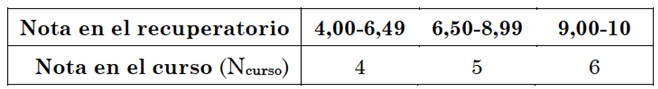
\includegraphics[scale=0.6]{Magistrales O_2020/notarecup.jpg}
\end{frame}

%\begin{frame}
%\frametitle{¿Uso de tecnología en magistrales?}
%\begin{itemize}
%    \item La tecnología puede ser buena en clase...
%    \item …pero hay evidencia creciente que sugiere que afecta en forma negativa a los estudiantes: para el que la usa y para el que está junto al que la usa!!!  
%    \item Vamos a aplicar una moderada restricción:
%laptops, tablets y celulares sólo en las últimas filas.
%\end{itemize}
%\end{frame}

\begin{frame}
\frametitle{Comunicación}
\begin{itemize}
    \item Prácticamente toda la información relevante del curso va a estar disponible en el Campus Virtual
    \item Consulten el Campus Virtual en forma regular
    \item ¡Hablen! Pregunten en clase a los instructores
    \item Contáctennos por correo electrónico 
\end{itemize}
\end{frame}

\begin{frame}
\frametitle{Feedback sobre las clases}
\begin{itemize}
    \item Realmente nos interesa saber como va el curso!!! \vspace{2mm}
    \item 2 opciones: \vspace{2mm}
        \begin{itemize}
            \item Nos pueden enviar un mail y contarnos que piensan 
            \item Nos pueden contestar una encuesta anónima que no podremos rastrear... Por supuesto, no podremos responder a estos mensajes!
  
        \end{itemize}
\end{itemize}
\end{frame}

\begin{frame}
\frametitle{Plagio y deshonestidad intelectual}
\small{
    La Universidad de San Andrés exige un estricto apego a los cánones de honestidad intelectual. La existencia de plagio configura un grave deshonor, impropio en la vida universitaria. Su configuración no sólo se produce con la existencia de copia literal en los exámenes sino toda vez que se advierta un aprovechamiento abusivo del esfuerzo intelectual  - ajeno. El Código de Ética de la Universidad considera conducta punible la apropiación de labor intelectual ajena desmereciendo los contenidos de novedad y originalidad que es dable esperar en los trabajos requeridos. La presunta violación a estas normas dará lugar a la conformación de un Tribunal de Ética que, en función de la gravedad de la falta, recomendará sanciones disciplinarias que pueden incluir el apercibimiento, la suspensión o expulsión.}
\end{frame}

\begin{frame}
\frametitle{Estructura del programa}
\begin{itemize}
\begin{itemize}
    \item Introducción
    \item Escasez y elección
    \itemInteracciones sociales
    \item Instituciones, poder, ganadores y perdedores
    \item Dentro de la firma
    \item Firmas eligiendo precio y cantidad
    \item Tomando precios
    \item Mercado laboral
    \item Crédito, dinero y bancos
    \item Fallas de mercado
    \item Fluctuaciones económicas
    \item Política fiscal
    \item Política monetaria
\end{itemize}
\end{itemize}
\end{frame}

\begin{frame}
\frametitle{Ahora si podemos comenzar...}
\centering
\huge
¡ BIENVENIDOS \\ \vspace{3mm} a \\ \vspace{3mm} ECONOMIA I !
\end{frame}


\end{document}


